\documentclass[article,a4paper,12pt,brazil,sumario=tradicional]{abntex2}
\usepackage{titlesec}

\setcounter{secnumdepth}{4}

\titleformat{\paragraph}
{\normalfont\normalsize}{\theparagraph}{1em}{}

\usepackage{array}
\usepackage{subfig}
\usepackage[utf8]{inputenc}
\usepackage{indentfirst}
\usepackage{hyperref}
\usepackage[hyphenbreaks]{breakurl}
\usepackage[alf,abnt-etal-text=it]{abntex2cite}
\usepackage[brazil]{babel}
\usepackage[space]{grffile}
\graphicspath{ {./images/} }
\setlength{\parindent}{3em}

\newcolumntype{C}[1]{>{\centering\arraybackslash\hspace{0pt}}p{#1}}

\setlrmarginsandblock{3cm}{3cm}{*}
\setulmarginsandblock{3cm}{2cm}{*}
\checkandfixthelayout

\titleformat{\section}{\normalfont\normalsize\bfseries}{\thesection.}{1em}{\MakeUppercase}
\titleformat{\subsection}{\normalfont\normalsize}{\thesubsection.}{1em}{\MakeUppercase}
\titleformat{\subsubsection}{\normalfont\normalsize\bfseries}{\thesubsubsection.}{1em}{}

\renewenvironment{quotation}
  {\small\list{}{\rightmargin=0cm \leftmargin=2cm}%
   \item\relax}
  {\endlist}
  
\hypersetup{%
    pdfborder = {0 0 0}
}

\title{ {\Large Título\footnote{Trabalho de conclusão de curso apresentado ao curso de Bacharelado em Sistemas de Informação da Universidade Federal Fluminense como requisito parcial para conclusão do curso.}\\\\
\vspace{.2} 
\textit{Titulo}\\}}

\date{ }

\begin{document}

\textual

\begin{center}
{\Large Título em português\footnote{Trabalho de conclusão de curso apresentado ao curso de Bacharelado em Sistemas de Informação da Universidade Federal Fluminense como requisito parcial para conclusão do curso.}

\textit{Comparativo de custo de tratamento para epilepsia no estado do Rio de Janeiro}\\}
\end{center}
\vspace{.2cm} 

\begin{flushright}
Bruno Moraes Cotelo\footnote{Graduando do Curso de Sistemas de Informação - UFF, bruno\_cotelo@id.uff.br}

Tiago Rodrigues de Matos\footnote{Graduando do Curso de Sistemas de Informação - UFF, ti\_matos@id.uff.br}

Daniel Cardoso Moraes de Oliveira\footnote{Orientador - Instituto de Computação - UFF, danielcmo@ic.uff.br.} 

Nome completo do coorientador\footnote{Coorientador - vínculo institucional do coorientador, e-mail do coorientador.}
\end{flushright}

\vspace{\onelineskip}

\begin{center}
    \textbf{Resumo}
\end{center}

\vspace{-.3cm}

\noindent Este estudo aprofundado investiga os custos do tratamento da epilepsia no Rio de Janeiro entre 2014 e 2023, focando no sistema público de saúde (SIASUS). O objetivo principal é comparar os custos do tratamento convencional com medicamentos antiepilépticos (MAEs) e o tratamento com canabidiol (CBD) em diferentes graus da doença..

\vspace{.4cm}
 
\noindent
\textbf{Palavras-chaves}: Epilepsia, Tratamento convencional, Canabidiol, Custos diretos, Custos indiretos, Graus da doença, Transições de estado, SIASUS, Rio de Janeiro.. 
 
\vspace{\onelineskip}

\begin{center}
    \textbf{Abstract}
\end{center}

\vspace{-.3cm}
\begin{hyphenrules}{english}
\noindent This comprehensive study delves into the intricate costs of epilepsy treatment in Rio de Janeiro between 2014 and 2023, with a specific focus on the public health system (SIASUS). The primary objective is to conduct a meticulous comparison of the financial implications associated with conventional treatment using antiepileptic drugs (AEDs) and the emerging alternative of cannabidiol (CBD) therapy, taking into account the varying degrees of epilepsy severity.
\end{hyphenrules}
\vspace{.4cm}
 
\noindent \textbf{Keywords}: Epilepsy, Conventional treatment, Cannabidiol, Direct costs, Indirect costs, Degrees of Disease, State transitions, SIASUS, Rio de Janeiro.

\vspace{.4cm}

\noindent \textbf{Aprovado em:} dd/mm/aaaa.~~~\textbf{Versão Final em:} dd/mm/aaaa

\section{Introdução}

\subsection{Epilepsia no SUS e Canabidiol}
A epilepsia se refere a um distúrbio da atividade cerebral caracterizado pela ocorrência periódica e espontânea de atividade elétrica altamente sincronizada, acompanhada de manifestações comportamentais. Dessa forma, não é uma única doença ou síndrome, e sim um grupo de distúrbios que ocorrem a partir de funções cerebrais alteradas. (Fonte: Alterações cardiovasculares e morte súbita nas epilepsias)

Essa complicação pode ocorrer motivada por diversos fatores, como febre, intoxicação, alterações vasculares ou doenças degenerativas. Atualmente, a epilepsia acomete cerca de 2\% da população brasileira, e cerca de 50 milhões de pessoas no mundo (Fonte GOV.BR (Na resolução da CONITEC diz 65M)). No Brasil é possível receber atendimento integral e gratuito pelo Sistema Único de Saúde (SUS), tendo 29 estabelecimentos habilitados para tratamento de alta complexidade em neurologia/neurocirurgia para abranger desde consultas, exames, diagnósticos, tratamento e fornecimento de medicamentos.

O uso de medicamentos para ajudar a controlar as crises faz com que os pacientes que sofrem dessa doença possam viver sem grandes limitações. Porém, cerca de 30\% desses pacientes ainda apresentam casos de crises, sendo considerados refratários ao tratamento. No SUS, segundo o Protocolo Clínico e Diretrizes Terapêuticas (PCDT) para epilepsia, publicado em 2018, são disponibilizados cerca de 13 medicamentos distintos para o tratamento, que deve ser iniciado com a prescrição de apenas um, podendo, em caso de falha, ser alterado ou feita a combinação de dois desses medicamentos antiepilépticos. (Fonte: Resolução CONITEC).

O canabidiol (CBD), um composto derivado da planta \textit{Cannabis sativa}, surge como uma alternativa promissora aos tratamentos convencionais. Evidências do uso medicinal da cannabis remontam a 5 mil anos atrás, com registros em diversas culturas como China, Índia, Egito, Grécia, Ásia e Oriente Médio. No uso comum, a planta era considerada sagrada ou com propriedades curativas.

Após séculos de uso tradicional e diversos estudos científicos, o CBD foi finalmente isolado na década de 40. Em 1963, a síntese do CBD foi concluída. Já o THC, canabinoide responsável pelos efeitos psicoativos e analgésicos, foi isolado em 1964 e sintetizado apenas em 1971. (Fonte: Cannabinoids and Epilepsy e Cannabis: 12.000 anos de experiências e preconceitos)

\subsection{Ciência de Dados}
Desde os primórdios da humanidade, registros foram criados por meio de gravuras e pinturas nas paredes e em objetos cotidianos. Com a invenção da escrita, a produção de dados e registros aumentou significativamente, tornando mais fácil difundir esses conhecimentos. No entanto, o verdadeiro salto ocorreu com a revolução digital e o surgimento dos computadores. Esse avanço exponencial permitiu a facilidade de armazenar uma quantidade avassaladora de informações e, a partir do processamento dessas informações, revelou o potencial dos dados para gerar conhecimento, identificar padrões, tomar decisões informadas e até fazer previsões. Como resultado, surgiu uma nova área de estudo: a ciência de dados.

A ciência de dados tem como objetivo criar valor a partir de processos de busca e conhecimento sobre os dados. Porém, por si só a ciência de dados não traz esse valor, é necessário um trabalho de análise desses dados para que se possa extrair o máximo deles o possível, e tornar a informação em algo objetivo que se possa ser utilizado.

Esta grande área de estudo, quando voltada para a área da saúde, pode ser utilizada para diversos fins, como auxílio no desenvolvimento de novos medicamentos, desenvolvimento de melhores estratégias de formulação de políticas públicas, porém destaca-se a divisão de 'dados clínicos' e 'dados de comportamento' para as análises. Os dados clínicos vêm de anotações médicas, resultados de exames e dados vindos de medidores. Tais informações são utilizadas para acompanhar o estado de saúde de pacientes e ajudar no diagnóstico. Os dados de comportamento monitoram as informações fisiológicas, como frequência cardíaca, qualidade de sono, respiração e informações oculares. Esses dados auxiliam na tentativa de prever distúrbios baseados nessas informações.

A recente liberação de novos medicamentos à base de canabidiol para o tratamento da epilepsia representa um marco significativo no cuidado da saúde pública. Esta medida não apenas oferece uma alternativa terapêutica promissora para pacientes que sofrem com crises refratárias, mas também tem o potencial de melhorar sua qualidade de vida. A introdução do canabidiol pode facilitar a transição de estados de saúde precários para uma condição mais estável e controlada. Além disso, ao considerar o impacto econômico, a adoção desses novos medicamentos pode representar uma mudança significativa nos custos associados ao tratamento da epilepsia.

O objetivo deste estudo é realizar uma análise comparativa dos custos de tratamento para a epilepsia no estado do Rio de Janeiro, no período de 2014 a 2023, a partir da análise dos dados clínicos disponibilizados pelo SUS, assim como dados de custo associados, investigando as diferenças entre os custos reais do tratamento convencional e as projeções de custo com a introdução do canabidiol como opção de tratamento. A análise buscará identificar potenciais economias ou custos adicionais em relação à adoção do canabidiol como parte do tratamento para pacientes com epilepsia refratária.

\section{Desenvolvimento}

\subsection{Metodologia}

Para inicio da analise foi necessario coletar os dados públicos no sistema do SIASUS. Com os arquivos extraidos, deu-se inicio ao processo de tratamento dos dados, que incluiu a concatenacao das bases anualmente, renomeacao de colunas, mapeamento de dados para tornar mais facil a leitura e aplicacao dos criterios de inclusao do grupo. Foi feita tambem uma analise exploratoria para entender melhor o cenário.

\begin{figure}[!ht]
    \centering
    \includegraphics[width=1\textwidth]{marcha_analitica.png}
    \caption{Marcha analítica do processo de analise dos dados}
    \label{fig:marcha_analitica}
    \end{figure}

\subsubsection{Coleta de dados}
A fonte primária do presente trabalho foi obtida por meio dos dados de dispensação de medicamentos do componente especializado da assistência farmaceutica que são enviados mensalmente para faturamento do programa em questão. Esses dados se tornam uma fonte útil de análise por serem públicos e possuírem dados atômicos de cada paciente a cada mês. O envio desta prestação de contas ao Ministério da Saúde é feito usando um documento chamado de APAC - Autorização de Procedimento de Alta Complexidade - que envolve o financiamento de programas de média e alta complexiade do SUS, incluindo transplantes e oncologia, bem como os medicamentos em questão. Destaca-se que a APAC gerada tem validade de 3 meses.
Os registros das APAC geradas a cada mês pelo sistema SIASUS foram utilizadas e extraídas do sítio apropriado(fonte) no formato DBC. Este é um formato compactado do arquivo do tipo DBF, originalmente utilizado pelo DBase. Estes arquivos podem ser tabulados utilizando o programa TabWin 4.1 que permite gerar consultas e extrair os dados com filtros de acordo com as condições necessárias e critérios de inclusão do estudo. Para realização das tabulações, também é necessário baixar os arquivos de extensão DEF, de definição, que permite modelar esta extração com os critérios necessários par ao estudo. 
No presente estudo foram filtradas as dispensações de medicamentos que estavam associadas ao CID G40.0 a G40.8 relativos à epilepsia e regulados pelo Protocolo Clínico e Diretrizes Terapêuticas da doença em questão. Apesar do arquivo de APAC ser elaborado mensalmente, as extrações foram agregadas anualmente em formato csv para posterior ingestão no sistema de análise.

\subsubsection{Tratamento dos dados}
 
A linguagem escolhida para trabalhar os dados foi Python, devido a sua rápida curva de aprendizado e grande variedade de bibliotecas disponiveis para manipulacao de dados e geracao de graficos. Alem do Python 3.x, foram utilizadas as bibliotecas Pandas para criacao de DataFrames para manipulacao, transformacao, analises dos dados e visualizacao, e a biblioteca Matplotlib para gerar graficos a partir dos DataFrames Pandas. 

Primeiramente, deve-se concatenar as bases, visto que os arquivos vem com os registros anuais. Dessa forma, o trabalho se concentra em apenas um DataFrame, facilitando as operacoes subsequentes. Foram encontrados 103.530 registros de consultas, distribuidos em 51 colunas de informacoes. Afim de diminuir o volume dos dados, foi feita uma curadoria para retirar colunas que sao irrelevantes para a analise, reduzindo de 51 colunas originais para apenas 24.

Em seguida, foram criados dicionarios de chave e valor, visando tanto renomear colunas quanto traduzir seus conteudos codificados para valores equivalentes, porem mais legiveis. Colunas com conteudo de procedimento, motivos de saida e permanencia, municipio e idade tiveram de ser mapeadas a partir das referencias dos dicionarios, que foram encontradas em (BUSCAR ONDE TAVA A FONTE).

\subsubsection{Criterios de inclusao}

O estudo incluiu todos os pacientes que continham registro a partir de abril de 2014 até setembro de 2023, considerando apenas os que iniciaram e finalizaram o tratamento dentro do periodo de tempo especificado. 

Foram excluidos os pacientes que continham dispensações registradas antes e depois das datas especificadas, pois dessa forma nao seria possivel precisar na analise informacoes sobre seu tratamento. Foram exluidos tambem os pacientes que possuiam menos de 3 dispensações no periodo analisado. 

Após a aplicacao dos criterios de inclusao, o numero de consultas registradas foi de 103.530 para 25.830, enquanto o numero de pacientes unicos foi de 5.509 para 2.123.

\subsubsection{Análise Exploratória}

Foi realizada um analise exploratória dos dados, afim de compreender melhor as caracteristicas da amostra. Dos pacientes unicos encontrados após aplicar os criterios de inclusao, 6.214 são menores de 18 anos, e 19.171 maiores de idade. A distribuicao dos sexos ficou em 1245 mulheres e 878 homens. É possível visualizar na Figura 2 a piramide etária dos pacientes:

\begin{figure}[!ht]
    \centering
    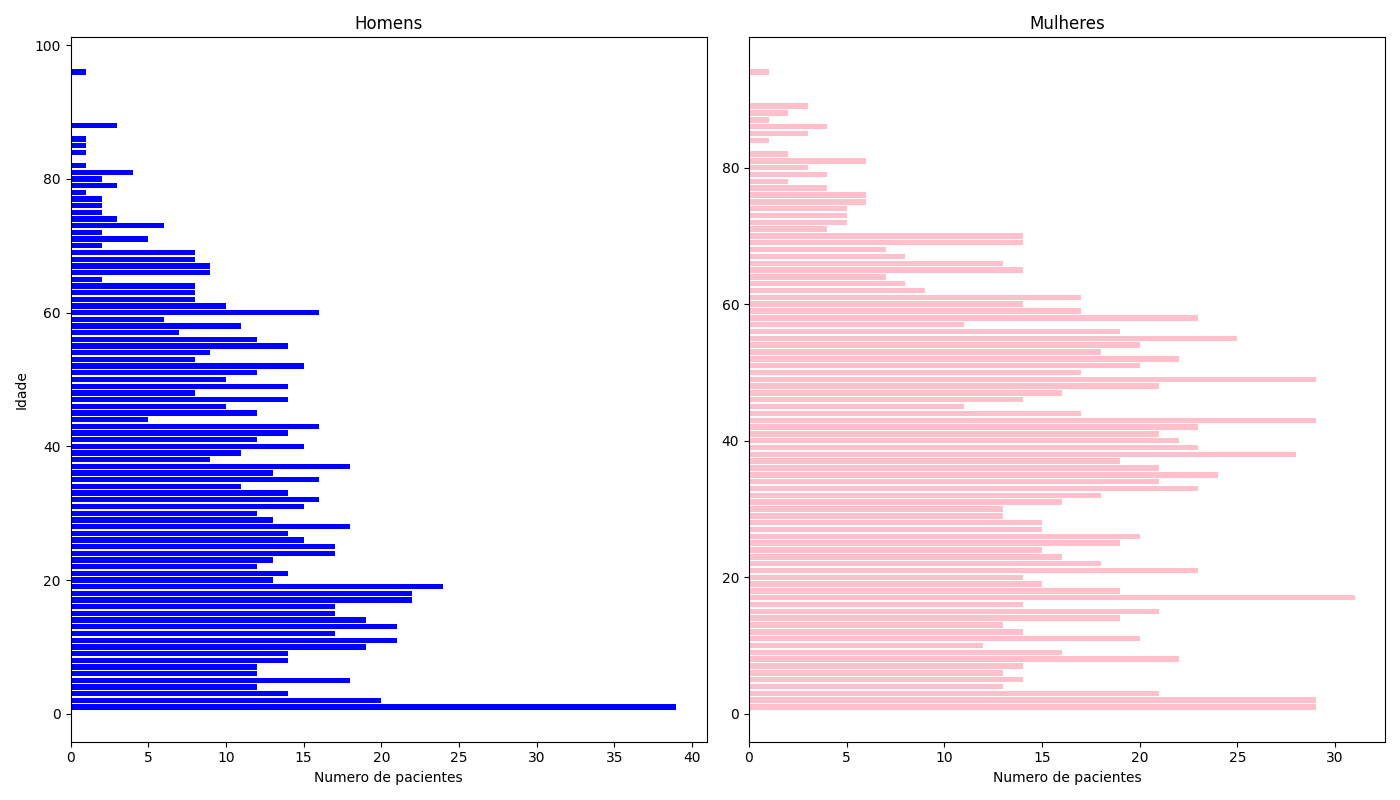
\includegraphics[width=1\textwidth]{piramide_etaria_completa.png}
    \caption{Piramide etária dos pacientes de epilepsia analisados.}
    \label{fig:piramide_etaria_completa}
    \end{figure}

Foram analisadas tambem particularidades sobre o tratamento utilizado. A dispensação total de material, distribuida entre os 5 medicamentos disponibilizados pelo SUS, ficou em:  

\begin{itemize}
    \item 9.315 Topiramato
    \item 1.969 Vigabatrina
    \item 4.709 Gabapentina
    \item 7.878 Lamotrigina
    \item 1.959 Levetiracetam
\end{itemize}

Ainda sobre o tratamento, foi extraido o numero de pacientes que iniciaram (Figura 3) e que sairam (Figura 4) do tratamento por ano, assim como o numero de trocas de procedimento (Figura 5).


    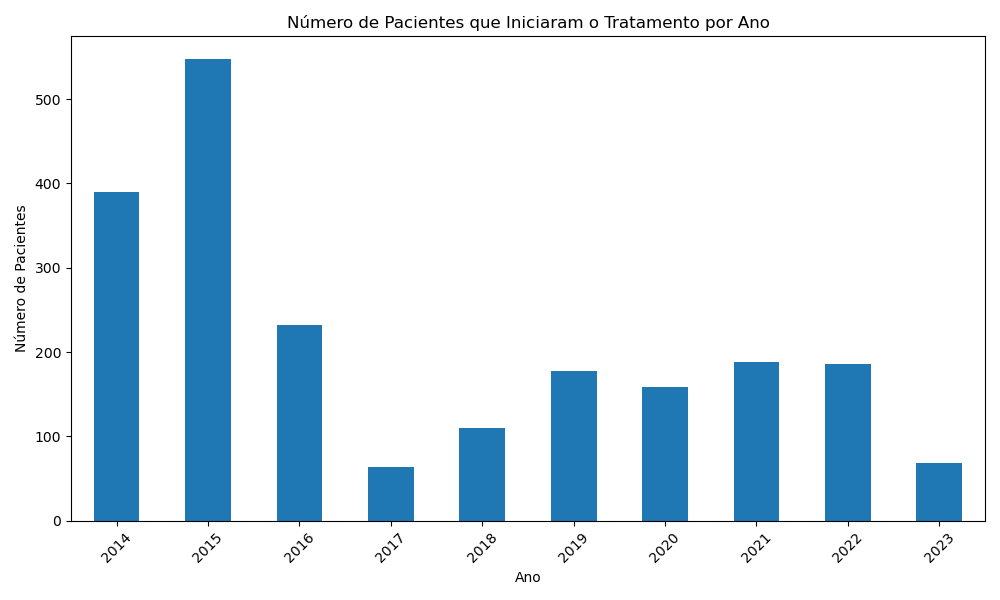
\includegraphics[width=1\textwidth]{pacientes_iniciaram_tratamento_por_ano.png}


    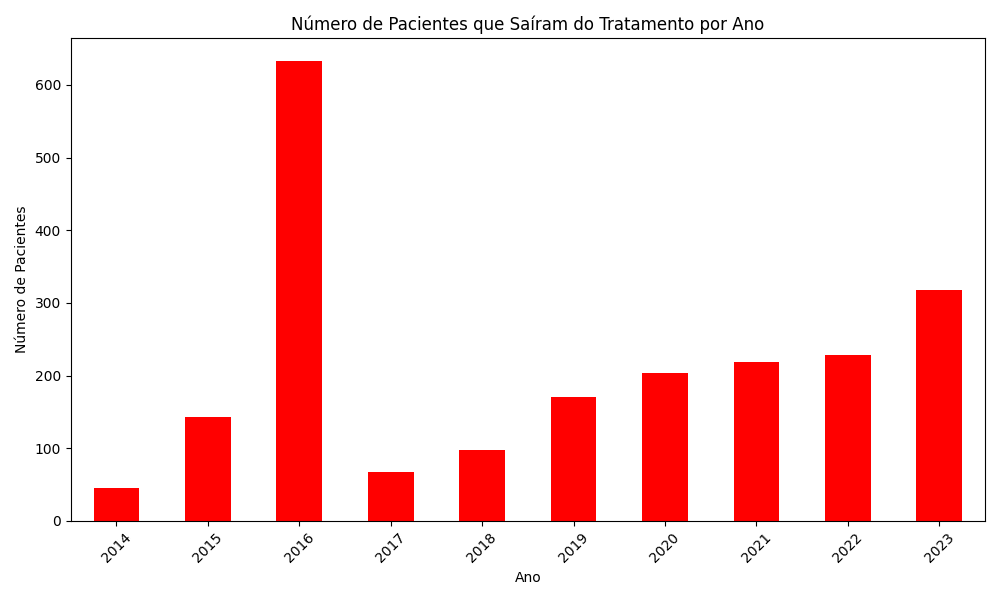
\includegraphics[width=1\textwidth]{pacientes_sairam_tratamento_por_ano.png}


    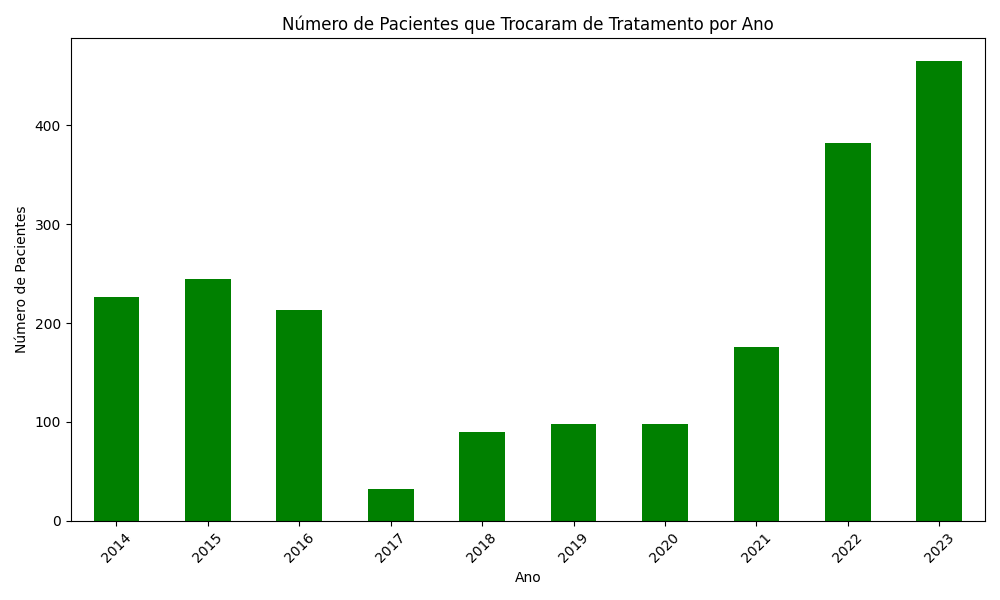
\includegraphics[width=1\textwidth]{pacientes_troca_tratamento_por_ano.png}




\subsubsection{Modelagem}

Modelagem

\subsection{Resultados}

\subsubsection{Analise descritiva}

Analise descritiva

\subsubsection{Modelagem}

Modelagem

\subsubsection{Custos}

Custos

\subsection{Discussao}

\section{Conclusao}

Parte final do artigo, na qual se apresentam as considerações correspondentes aos objetivos e/ou hipóteses.

\subsection{Citações}

As citações apresentadas no artigo seguirão as normas de apresentação de acordo com a NBR 10520:2002 ~\cite{bibliografica6023}. Para chamada das citações será adotado o sistema ``autor-dat'' em todo artigo. As chamadas incluídas na sentença devem ser em letras maiúsculas e minúsculas e, quando estiverem entre parênteses devem ser em letras maiúsculas. Nas citações diretas devem ser especificadas a(s) página(a) da fonte consultada; para citações indiretas este item é opcional. Todas as obras citadas deverão aparecer na lista de referências, e não, em notas de rodapé.

De acordo com Associação Brasileira de Normas Técnicas (~\citeyear{bibliografica6023}), ``as citações diretas, no texto, com até três linhas, devem estar contidas entre aspas duplas''.

\begin{quotation}
\noindent
As citações diretas, no texto, com mais de três linhas, devem ser destacadas com recuo de 4cm da margem esquerda, com letra menor que a do texto e sem aspas ~\cite{bibliografica6023}.
\end{quotation}

\subsection{Notas de rodapé}

As notas de rodapé devem ser utilizadas apenas para notas explicativas, ou seja, usadas para comentários, esclarecimentos ou explanações que não possam ser incluídos no texto. A numeração das notas é feita em algarismos arábicos, de forma única e consecutiva.

\subsection{Numeração progressiva}

A numeração progressiva das seções no desenvolvimento do artigo deve atender às especificações da ABNT NBR 6024:2012. As seções devem se limitar até a seção quinária e seus títulos devem ser destacados tipograficamente, de forma hierárquica, através de recursos gráficos de maiúscula, negrito, itálico ou sublinhado e outros.

\subsection{Figuras e tabelas}

Todas as figuras e tabelas devem ser numeradas em ordem crescente, na sequencia que são citadas no corpo do artigo. As figuras e tabelas devem ser exibidas preferencialmente logo após o parágrafo onde ela é citada. Todas as figuras e tabelas devem ser citadas no corpo do texto. O posicionamento da legenda é logo abaixo da figura, conforme exemplificado na Figura~\ref{fig:exampleFig1}.

\begin{figure}[!ht]
\centering
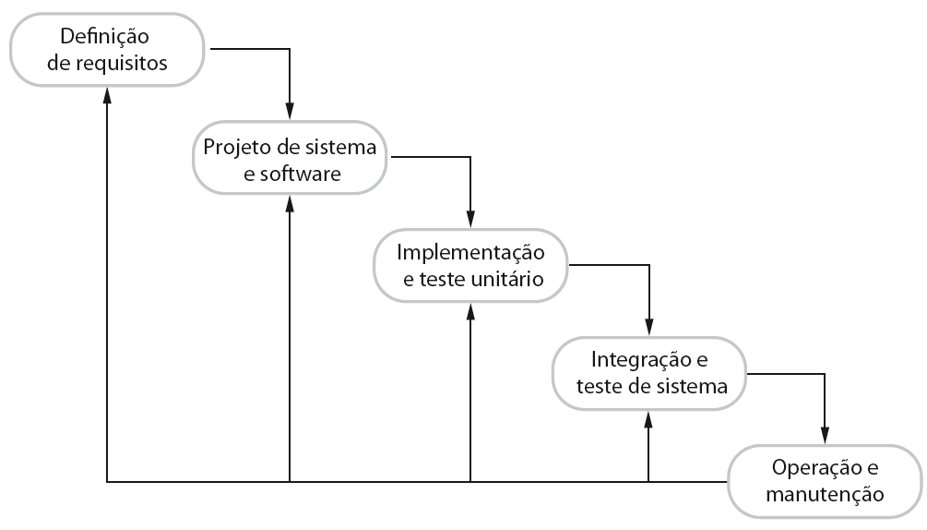
\includegraphics[width=1\textwidth]{Imagem1.png}
\caption{Modelo do processo de desenvolvimento de software em cascata. Fonte: \cite{sommerville2011software}.}
\label{fig:exampleFig1}
\end{figure}

Nas tabelas, tente evitar o uso de fundos coloridos ou sombreados e evite linhas de enquadramento grossas, dobradas ou desnecessárias. Ao relatar dados empíricos, não use mais dígitos decimais do que o garantido por sua precisão e reprodutibilidade. A legenda da tabela deve ser colocada acima da tabela (consulte a Tabela~\ref{tab:exTable1}).

\begin{table}[!ht]
\centering
\caption{Taxa de sucesso de projetos de desenvolvimento de software pelo tamanho do projeto. Fonte: \cite{clancy1995standish}.}
      \begin{tabular}{| p{3cm} | C{2cm} | C{2cm} | C{2cm} |}
        \hline
        & Bem sucedido & Deficitário & Falho \\ \hline
        Muito grande & 2 & 7 & 17 \\ \hline
        Grande & 6 & 17 & 24 \\ \hline
        Médio & 9 & 26 & 31 \\ \hline
        Pequeno & 21 & 32 & 17 \\ \hline
        Muito pequeno & 62 & 16 & 11 \\ \hline
        \textbf{TOTAL} & \textbf{100} & \textbf{100} & \textbf{100} \\ \hline
    \end{tabular}
    \label{tab:exTable1}
\end{table}

\subsection{Referências}

As referências bibliográficas devem ficar localizadas ao final do texto, contendo exclusivamente as obras citadas, ordenadas em uma única ordem alfabética e de acordo com as normas vigentes da ABNT NBR 6023/2018. Devem ser digitadas com espaçamento simples entre linhas e separadas entre si por um espaço simples em branco. O alinhamento do texto deve ser à esquerda.

A expressão ``Referências'' deve figurar de forma centralizada e não numerada, com o mesmo destaque tipográfico das seções primárias e logo após a conclusão.

Para esclarecimentos, consultar a norma correspondente.

\section{Conclusão}

Parte final do artigo, na qual se apresentam as considerações correspondentes aos objetivos e/ou hipóteses.

\newpage
\bibliography{references}

\newpage
\renewcommand{\listfigurename}{APÊNDICE A - Lista de ilustrações}
\listoffigures

\newpage
\renewcommand{\listtablename}{APÊNDICE B - Lista de tabelas}
\listoftables

\begin{appendices}
\newpage
\chapter* {APÊNDICE C}
\noindent
Os apêndices A e B devem conter a lista de ilustrações e tabelas, respectivamente. Os apêndices seguintes podem ser usados para apresentar textos elaborados pelo próprio autor, a fim de complementar a sua argumentação. Por exemplo, no caso de desenvolvimento de sistemas, podem constar nos apêndices os artefatos gerados da análise de sistemas, como protótipos de telas, casos de uso, diagramas UML, ou a lista de requisitos de negócio e de usuário.

\newpage
\chapter*{ANEXO A}
\noindent
Seção opcional. Anexos são os documentos de autoria externa, ou não elaborados pelo autor, que servem de fundamentação, comprovação ou ilustração.
\end{appendices}

\newpage
\chapter*{Agradecimentos}
\noindent
Seção opcional. Oportunidade para o(s) autor(es) registrar(em) os agradecimentos, em especial, quando o artigo recebeu ajuda financeira de alguma instituição de fomento, ou represente o resultado de um trabalho colaborativo ou multidisciplinar, envolvendo áreas externas ao Instituto de Computação.

\end{document}
